% Chapter 1

\chapter{Introducción general} % Main chapter title

\label{Chapter1} % Change X to a consecutive number; for referencing this chapter elsewhere, use \ref{ChapterX}


En este capítulo se explica brevemente el marco de trabajo en en el cual se desarrolla el proyecto y se dan las primeras definiciones sobre el equipo a construir. 
%----------------------------------------------------------------------------------------
%	SECTION 1
%----------------------------------------------------------------------------------------
\section{Tecsci sas}

La realización del siguiente proyecto se basa en la construcción de un equipo comercial \textit{Dip Coater}. El proyecto se desarrolla en el marco de los primeros años de vida de la empresa \textit{TECSCI (Technology for Science)}.

La empresa tiene como visión ser líder y referente global en el desarrollo de equipamiento científico de fuentes abiertas y como misión 
pretende fabricar productos innovadores de alta calidad para atender las demandas de los laboratorios de investigación, universidades y empresas de base tecnológica nacionales e internacionales.

Con el objetivo general de diseñar y fabricar equipos con foco en procesos nanotecnológicos, adhiriendo a la filosofía del software y hardware libre y aportando desde su lugar a la comunidad. El Dip coater es el primer equipo realizado y se adapta completamente al modelo de negocio pensado, el cual se presenta en la Figura \ref{fig:diagBloques} en donde se describe el modelo de negocios de la empresa sobre un diagrama Canvas.

\clearpage

\vspace{1cm}
\begin{figure}[htpb]
\centering 
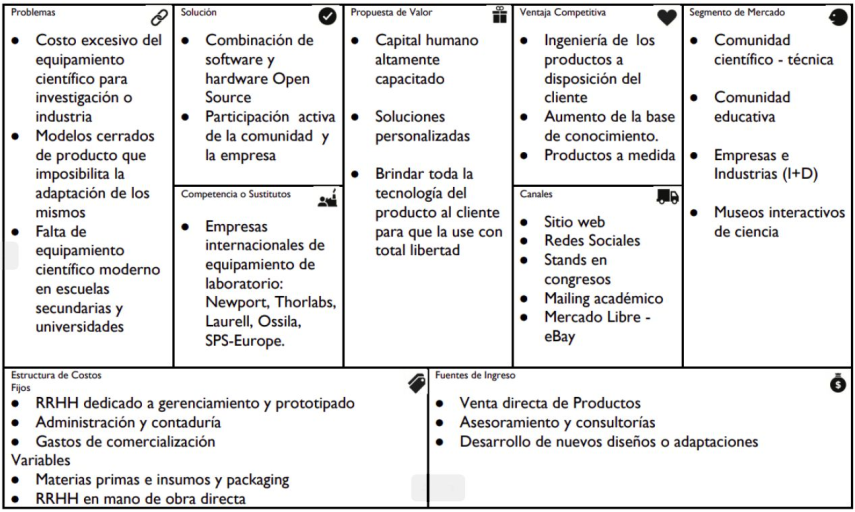
\includegraphics[width=1\textwidth]{./Figures/canvas.png}
\caption{Diagrama Canvas - Modelo de Negocios TECSCI}
\label{fig:diagBloques}
\end{figure}
\vspace{1cm}


Las soluciones que propone Tecsci se orientan a dar respuesta a las problemáticas que se comparten tanto en el mercado local como en el internacional:
\begin{itemize}
\item Elevado precio del equipamiento científico y mantenimiento.
\item Contratación exclusiva de servicio técnico asociado al fabricante.
\item Soluciones de software y hardware cerradas que no permiten la adaptación del instrumental a experimentos científicos personalizados.
\end{itemize}

%-----------------------------------
%	SUBSECTION 1
%-----------------------------------

\section{Dip coating}


En los laboratorios de investigación aplicados a nanotecnologías existen diferentes equipos para la fabricación de películas delgadas comunmente denominadas \textit{thin film}, las películas delgadas son finas capas de material de espesores variables que comunmente van desde las centenas de nanómetros hasta las decenas de micrones \textit{[100nm - 50 um]} que se depositan sobre diferentes superficies.  

Para la creación de películas delgadas por deposición se utilizan diferentes tipos de técnicas físicas o químicas, también existe la posibilidad utilizando otro tipo de técnicas de hacer crecer la película sobre la superficie.
Se utilizará para este proyecto la técnica de inmersión controlada de una superficie de muestra en un sustrato disuelto en solución.

Dip Coating es una técnica que se emplea tanto en áreas de I+D en la industria, como en la investigación científica en el campo de las nanociencias, se basa en la inmersión y extracción de una muestra en una solución bajo estudio, como se observa en la Figura \ref{fig:inmersion} en donde se observa una ejecución completa del movimiento desarrollado por el equipo.

\vspace{1cm}
\begin{figure}[htpb]
\centering 
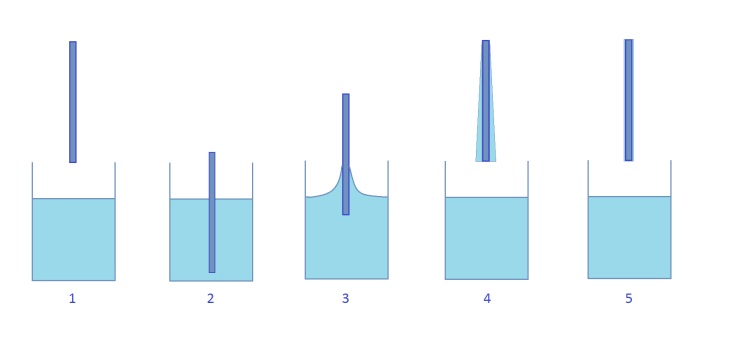
\includegraphics[width=0.9\textwidth]{./Figures/dip-coating.png}
\caption{Proceso completo desarrollado por el equipo}
\label{fig:inmersion}
\end{figure}
\vspace{1cm}
 
La principal y mas importante característica de la máquina es darle al usuario la posibilidad de controlar la velocidad y aceleración de inmersión de la muestra, el tiempo de espera en que la muestra queda sumergida, y también controlar la extracción, teniendo la posibilidad de repetir el ciclo según se desee.
 

%-----------------------------------
%	SUBSECTION 2
%-----------------------------------

\section{Estado del arte}

Existen diferentes fabricantes a nivel mundial que comercialízan estos equipos pero ninguno a nivel local, también podemos encontrar diferentes modelos dip coater, por ejemplo la empresa Biolin Scientific tiene una versión simple y también ofrece version mas compleja, presentamos a continuación algunos equipos de diferentes fabricantes.

\textbf{Biolin Scientific}  \citep{1_web_biolin}

En la figura \ref{fig:equipos_biolin} podemos ver el equipo simple que ofrece la companía y otro mas avanzado que a través de una rotación en la base cambia automáticamente las soluciones donde se realizan las inmersiones. Ambos equipos necesitan estar conectados a una pc corriendo un software para poder ser ejecutados.

\begin{figure}[!htpb]
     \centering
     \begin{subfigure}[b]{0.4\textwidth}
         \centering
         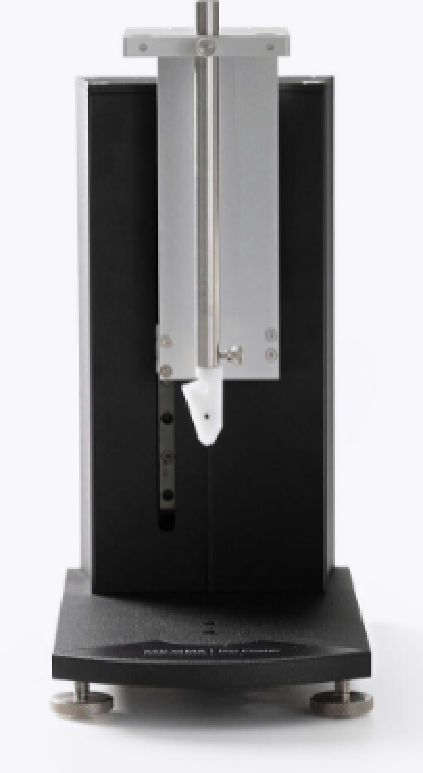
\includegraphics[width=.65\textwidth]{./Figures/dip_biolin.pdf}
         \caption{Equipo simple}
         \label{fig:dip_biolin}
     \end{subfigure}
     \hfill
     \begin{subfigure}[b]{0.4\textwidth}
         \centering
         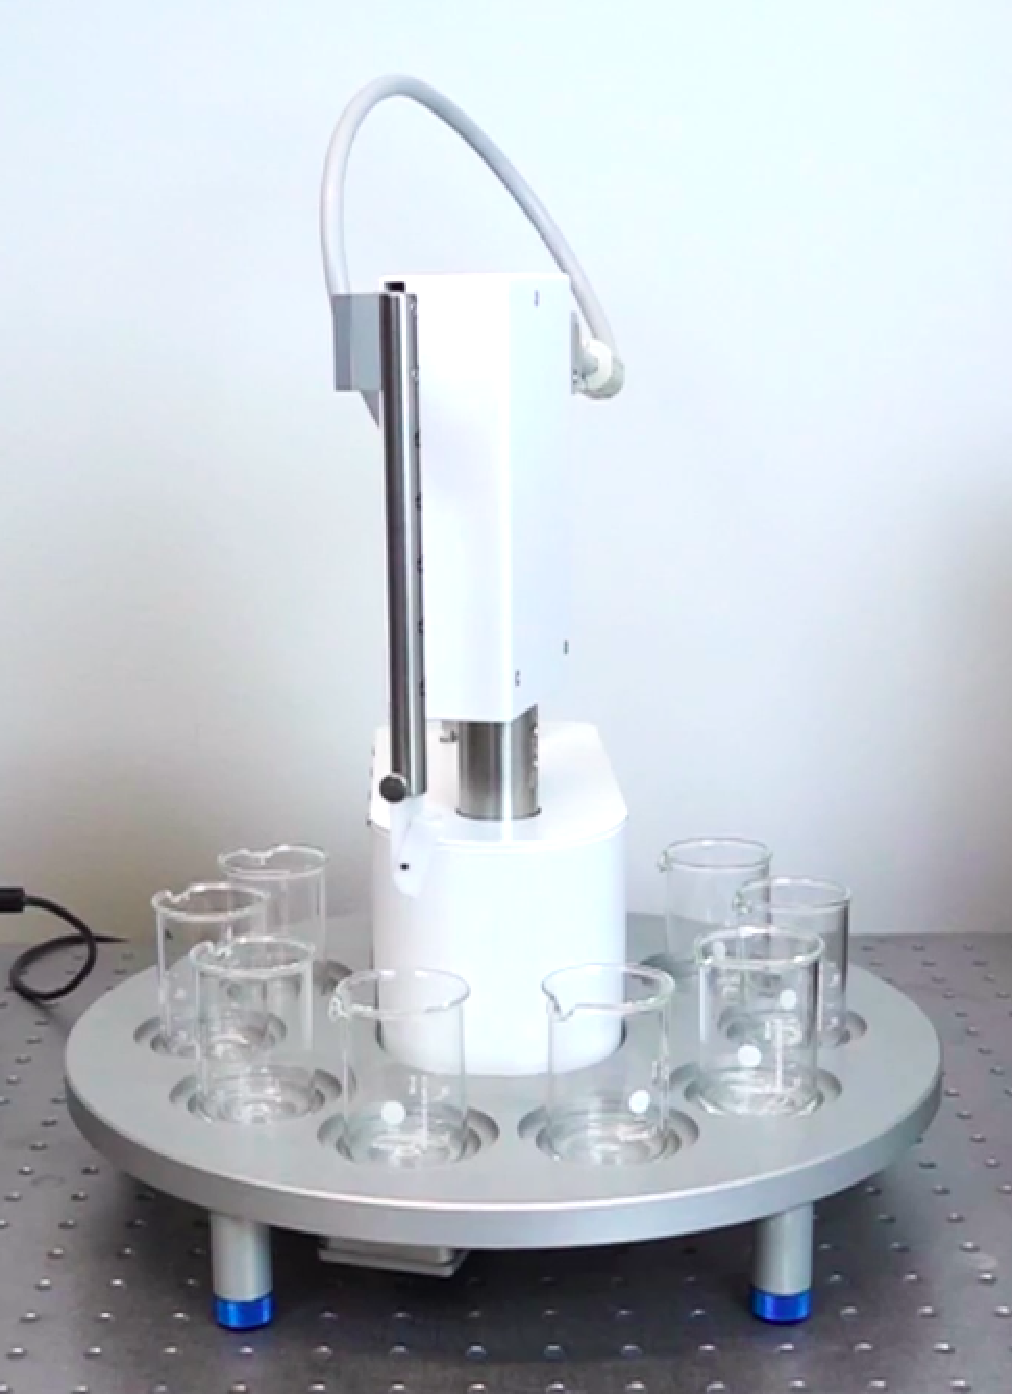
\includegraphics[width=.85\textwidth]{./Figures/dip_biolin_2.pdf}
         \caption{Equipo avanzado}
         \label{fig:dip_biolin_2}
     \end{subfigure}
     \hfill
        \caption{Equipos de la empresa Biolin Scientific}
        \label{fig:equipos_biolin}
\end{figure}



\textbf{Kibron}  \citep{2_web_kibron}

\ref{fig:dip_kibron}

\begin{figure}[htbp]
	\centering
	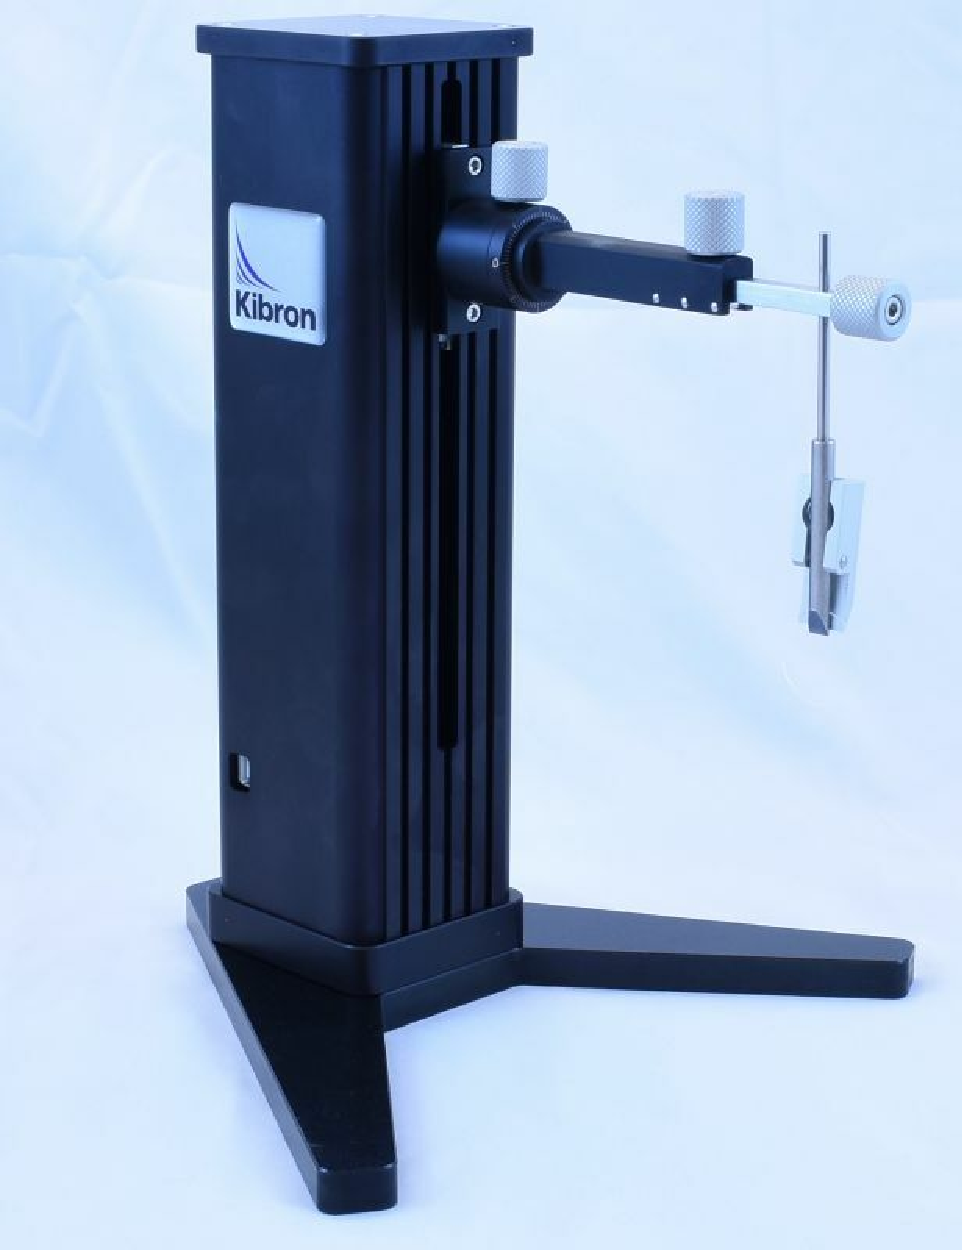
\includegraphics[width=.35\textwidth]{./Figures/kibron.pdf}
	\caption{Equipo de la empresa Kibron.}
	\label{fig:dip_kibron}
\end{figure}

\textbf{Ossila}  \citep{4_web_ossila}

y luego en la siguiente tabla \ref{tab:equipos_competencia} comparamos las especificaciones técnicas que los caracterizan.

\begin{table}[h]
	\centering
	\caption[caption corto]{Especificaciones técnicas de otros fabricantes}
	\begin{tabular}{l c c c}    
		\toprule
		\textbf{Equipo} 	 & \textbf{Recorrido max.}  & \textbf{Velocidad (mm/min)}  & \textbf{Acel (m/min2)}\\
		\midrule
		Bio Single Vessel Medium	& 300 mm 	& 1    - 1000   & without 		\\		
		Bio Multiplie Vessel		& 70  mm	& 0.1  - 108 	& without		\\
		Kibron LayerX				& 134 mm	& 0.06 - 300	& without		\\
		Ossila						& 100 mm	& 0.6 - 3000	& without		\\
		\bottomrule
		\hline
	\end{tabular}
	\label{tab:equipos_competencia}
\end{table}

%----------------------------------------------------------------------------------------
%	SECTION 3
%----------------------------------------------------------------------------------------

\section{Objetivos y alcance}

\subsection{Objetivos}

El objetivo de este proyecto es que la empresa TECSCI diseñe y fabrique el primer equipo comercial, con la perspectiva de ser el primero de una serie más amplia de equipos de laboratorio para la investigación científica. En principio el proyecto se enmarca en la temática de estudio sobre aplicaciones  Nanotecnologícas, pero el campo al cual se apunta es mucho más amplio, y se pretende poder abarcarlo incrementalmente respetando los principios filosóficos del Hardware y Software Libre.


\subsection{Alcance}

El presente proyecto incluye la presentación de un equipo comercial Dip Coater. 

Abarca los siguientes puntos:

\begin{itemize}
\item Desarrollo del Firmware que contemple la comunicación con driver del fabricante TRINAMIC, específicamente el TMC5130.
\item Diseño del Hardware con software de diseño KICAD.
\item Fabricación del PCB y montaje de componentes electrónicos.
\item Diseño y Fabricación de la parte mecánica soporte del equipo y fabricación de piezas especiales a través de mecanizado CNC.
\item Incorporación de pantalla touch HMI \textit{human machine interface} de la marca STONE para configuración y uso del equipo.
\end{itemize}



El presente proyecto no incluye:

\begin{itemize}
\item Desarrollo de hardware con fuente de alimentación incorporada.
\item Programación de la interfaz gráfica con el software de diseño provisto por el fabricante de la pantalla.
\item Control del entorno con registro de humedad, temperatura y  cámara de humedad.
\end{itemize}



